
\documentclass[12pt]{article}
\usepackage{amsmath}
\DeclareMathOperator*{\argmin}{arg\,min} % thin space, limits underneath in displays
\DeclareMathOperator*{\argmax}{arg\,max} % thin space, limits underneath in displays
\newtheorem{thm}{Theorem}
\usepackage{amssymb}
\usepackage{amsfonts}
\usepackage{mathrsfs}
\usepackage{bm}
\usepackage{indentfirst}
\setlength{\parindent}{0em}
\usepackage[margin=1in]{geometry}
\usepackage{graphicx}
\usepackage{setspace}
\doublespacing
\usepackage[flushleft]{threeparttable}
\usepackage{booktabs,caption}
\usepackage{float}
\usepackage{graphicx}
\usepackage[sort,comma]{natbib}
\usepackage[hidelinks]{hyperref}

\usepackage{import}
\usepackage{xifthen}
\usepackage{pdfpages}
\usepackage{transparent}

\newcommand{\incfig}[1]{%
\def\svgwidth{\columnwidth}
\import{./figures/}{#1.pdf_tex}
}




\title{The Solow Growth model}
\author{}
\date{}


\begin{document}
\maketitle

{\textbf {Conclusion:}}

the accumulation of physical capital cannot account for (explain) either the vast 
growth over time in output per person, $ g_{\frac{Y}{L}} $, or the vast geographic 
differences in output per person.

The model treats other potential sources of differences in real incomes, $ Y $, as
either exogenous (e.g., technological progress) or absent altogether (e.g., positive 
externalities from capital).

It does not investigate the determinants of saving and investment.



\section{Assumptions}



\subsection{Four variables: }
\begin{itemize}
\item output, $ Y $
\item capital, $ K $
\item labor, $ L $
\item knowledge, or the effectiveness of labor, $ A $
\end{itemize}


Ignore other inputs, e.g., natural resources.



\subsection{Production function:}

\subsubsection{Labor-augmenting}
\begin{equation*}
Y(t) = F[K(t), A(t)L(t)]
\end{equation*}

It says technology progress is labor-augmenting or Harrod-neutral.

================================\\
Note:\\
Technology progress is capital-augmenting if $ Y = F(AK,L) $\\
Technology progress is Hicks-neutral if $ Y = AF(K,L) $\\
================================


\subsubsection{CTRS}
Production function is constant return to scale in $ K $ and $ AL $. 
\begin{equation*}
F(\lambda K, \lambda AL) = \lambda F(K, AL),\quad \forall \lambda \ge 0.
\end{equation*}

If we let $ \lambda = \frac{1}{AL} $,
\begin{align*}
F \left( \frac{K}{AL},1 \right)  &= \frac{1}{AL}F(K,AL)\\
\frac{K}{AL}&: \text{ capital per effective labor }\\
\frac{1}{AL}F(\cdot ) = \frac{Y}{AL}&: \text{ output per effective labor }
\end{align*}

Define:
\begin{align*}
k &= \frac{K}{AL}\\
y &= \frac{Y}{AL}\\
y &= f(k) = F(k,1) = F \left( \frac{K}{AL},1 \right) = \frac{1}{AL}F(K,AL)\\
\frac{Y}{L}&= A \left( \frac{Y}{AL} \right)  = Af(k)
\end{align*}

\subsubsection{Quasi-concave}
For $ f(k) $,
\begin{equation*}
f(0) = 0, \quad f'(k) > 0, \quad f''(k) < 0
\end{equation*}

Since 
\begin{equation*}
F(K,AL) = AL f(K/AL),
\end{equation*}
the MPK would be
\begin{align*}
MPK &= AL f'\left( \frac{K}{AL} \right) \frac{1}{AL} = f' (k) > 0.
\end{align*}

And
\begin{align*}
\lim_{k \to \infty} f'(k) &= 0\\
\lim_{k \to 0} f'(k) &= \infty 
\end{align*}


Consider a Cobb-Douglas production function
\begin{equation*}
F(K,AL) = K^{\alpha}(AL)^{1 - \alpha}, \quad \alpha \in (0,1)
\end{equation*}
\begin{align*}
f(k)&= F \left( \frac{K}{AL}, 1 \right) \\
&= \left( \frac{K}{AL} \right) ^{\alpha}\\
&= k ^{\alpha}\\
f'(k)&= \alpha k ^{\alpha - 1}
\end{align*}




\section{Accumulation of inputs}
$ K_0, L_0, A_0 $ are given and strictly positive.

Growth rate of $ L $ and $ A $
\begin{align*}
\dot{L}(t)&= nL(t)\\
\dot{A}(t)&= gA(t),
\end{align*}
where $ n,g $ are exogenous.

{\textbf {Capital accumulation}}
\begin{equation*}
		\dot{K}(t)  = [Y(t) - C(t)] - \delta K(t) = I(t) - \delta K(t)
\end{equation*}

\noindent\fbox{%
\parbox{\textwidth}{%
The only substantial differences among Solow, Ramsey, and Diamond overlapping-
generations model concern their assumptions about how output is divided between
Consumption and Investment.

In both Ramsey and Diamond models, divisions arises endogenously.
}%
}\\


In the Solow model, the division is taken as given, the exogenous saving rate ($ s $).
\begin{equation*}
\dot{K}(t) = sY(t) - \delta K(t), \quad s \in (0,1]
\end{equation*}




Recall, $ k(t) = K(t)[A(t)L(t)]^{ - 1} = \frac{K(t)}{A(t)L(t)} $, then
\begin{align*}
\frac{dk(t)}{dt} = \dot{k}(t)
&= \dot{K}(t)[A(t)L(t)]^{ - 1} - K(t)[A(t)L(t)]^{ - 2}[\dot{A}(t)L(t) + A(t)\dot{L}(t)]
\\
&= \frac{\dot{K}}{AL} - \frac{K}{(AL)^{2}}\dot{A}L - \frac{K}{(AL)^{2}}A\dot{L}\\
&= \frac{\dot{K}}{AL} - \frac{K}{AL}\frac{\dot{A}L}{AL} - \frac{K}{AL}\frac{A\dot{L}}{
AL}\\
&= \frac{\dot{K}}{AL} - \frac{K}{AL}\frac{\dot{A}}{A} - \frac{K}{AL}\frac{\dot{L}}{L}\\
&= \frac{sY - \delta K}{AL} - kg - kn, \quad 
\text{ since $ \dot{K} =  sY - \delta K$ }\\
&= \frac{sY}{AL} - k \delta - kg - kn\\
\dot{k}&= sf(k) - (\delta + g + n)k
\end{align*}
This is the key equation of the Solow model.

\begin{figure}[H]
\center{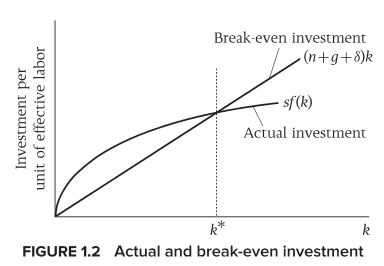
\includegraphics[scale =.8 ]  {figures/solow_investment_actual-break-even.png}}
\end{figure}

If $ k < k ^{*} $ , actual investment is greater than the break-even investment, so
$ k $ is rising.

$ k $ converges to $ k ^{*} $.


\section{Balanced growth path}

\begin{equation*}
k = \frac{K}{AL} \rightarrow K = ALk, \quad g_{K} = g_{A} + g_{L} + 0 = g + n
\end{equation*}

When $ k = k ^{*} $, $ k $ is constant,

$ K $ grows at rate $ g + n $,

$ \frac{Y}{L} $ grows at rate $ g $

The Solow model implies that {\textbf {regardless of its starting point, the economy
converges to a balance path--a situation where each variable is growing at a constant
rate. The growth rate of output per worker, $ \frac{Y}{L} $, is determined solely
by the rate of technological progress, $ g $.}}


\subsection{The impact of a change in the saving rate}
\subsubsection{The impact on output}

\begin{figure}[H]
\center{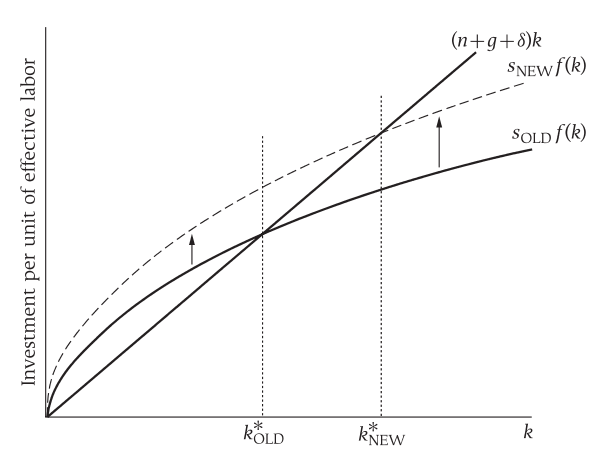
\includegraphics[scale =.5 ]  {figures/change_in_saving.png}}
\end{figure}

\begin{figure}[H]
\center{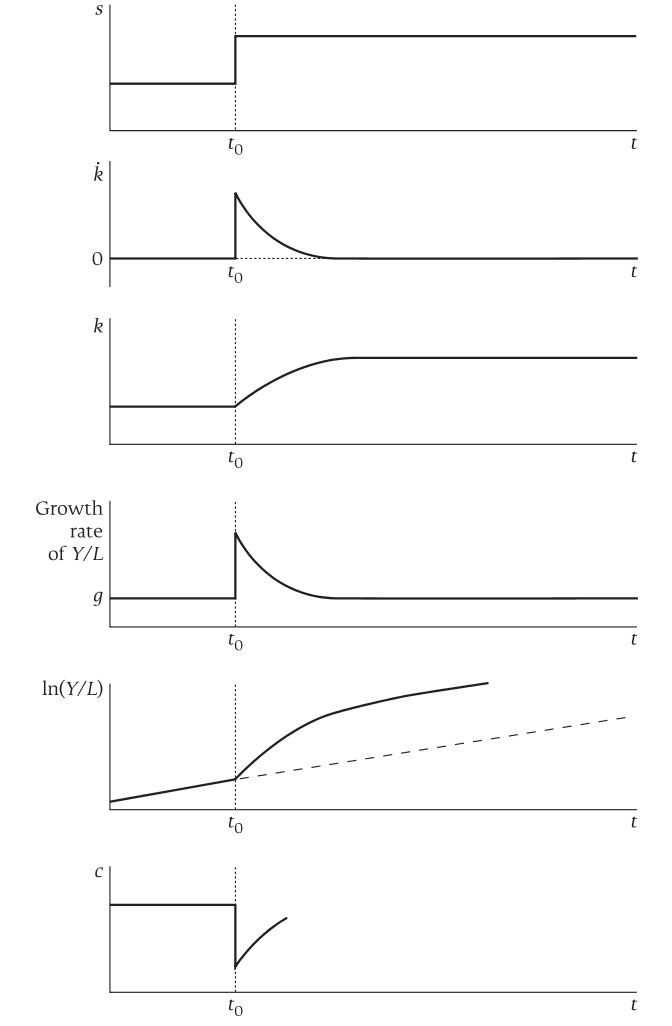
\includegraphics[scale =.5 ]  {figures/solow_impact_saving.png}}
\end{figure}

The growth rate of $ \frac{Y}{L} $:
recall $ \frac{Y}{L} = Af(k) $, a permanent increase in $ s $ causes $ k $ to increase,
hence, $ \frac{Y}{L} $ grows both because $ A $ and $ k $. It follows the path
of $ \dot{k} $ because when $ k $ approach to new SS, $ \dot{k} = 0 $, so $ \frac{Y}{L}
$ goes back to previous growth rate, $ g $.

Hence, change in the saving rate has a {\textbf {level effect}}, but not a 
{\textbf {growth effect}}.


\subsubsection{The impact on consumption}

Recall, $ c = (1 - s)f(k) $, $ c $ is consumption per effective labor.

If $ s $ permanently goes up, $ c $ jumps down immediately, and then rises gradually
as $ k $ is growing to the new SS level.

Given the first two equations below, we can derive the $ c^{*} $ at SS as a function
of $ k ^{*} $
\begin{align*}
c^{*} &= f(k ^{*}) - sf(k ^{*})\\
sf(k ^{*}) &= (n + g + \delta)k ^{*}\\
c^{*} &= f(k ^{*}) - (n + g + \delta)k ^{*}
\end{align*}

Recall that $ k ^{*} $ is a function of $ n, g, \delta, s $. We can find the impact
of $ s $ on $ c^{*} $ by differentiating $ c^{*} $ wrt $ s $.
\begin{align*}
\frac{\partial c^{*} }{\partial s }&= f'(k ^{*})\frac{\partial k ^{*} }{\partial s }
 - (n + g + \delta) \frac{\partial k ^{*} }{\partial s }\\
&= [f'(k ^{*}) - (n + g + \delta)]\frac{\partial k ^{*} }{\partial s }
\end{align*}
The golden-rule $ k $, is determineby 
\begin{equation*}
f'(k ^{*}) = (n + g + \delta)
\end{equation*}

We know $ \frac{\partial k ^{*} }{\partial s } > 0 $. Hence,

if  $ f'(k ^{*}) < (n + g + \delta) $, invest more, so, $ c $ goes down.

if  $ f'(k ^{*}) > (n + g + \delta) $, invest less, so, $ c $ goes up.

if  $ f'(k ^{*}) = (n + g + \delta) $, a marginal change in $ s $ has no effect on 
$ c $.
These three scenarios above is shown in figures below:\\

\newpage

Case 1: $ f'(k ^{*}) < (n + g + \delta) $
\begin{figure}[ht]
    \centering
    \incfig{mpk-less-than-breakeven-level}
    \caption{mpk less than breakeven level}
    \label{fig:mpk-less-than-breakeven-level}
\end{figure}

Recall, $ c = f(k) - (n + g + \delta)k $, hence the distance between these two curves
is the consumption level per effective labor.

It shows that if $ f'(k ^{*}) < (n + g + \delta) $, a rise in $ s $ will cause a 
decrease in consumption.\\




Case 2: $ f'(k ^{*}) > (n + g + \delta) $
\begin{figure}[ht]
    \centering
		\scalebox{.7}{\incfig{mpd-greater-than-breakeven-level}}
    \caption{mpd greater than breakeven level}
    \label{fig:mpd-greater-than-breakeven-level}
\end{figure}

It says if $ f'(k ^{*}) > (n + g + \delta) $, a rise in $ s $ will cause an increase in
consumption.



\section{Long-run equilibrium}
Now we want to measure the effect of a change of $ s $ on the output $ y $.
So we want to find $ \frac{\partial y^{*} }{\partial s } $.

Recall, 
\begin{equation*}
y = f(k), \quad y^{*} = f(k ^{*}) \rightarrow y^{*} = f(k ^{*}(s,n,g,\delta))
\end{equation*}
Differentiate $ y^{*} $ wrt $ s $,
\begin{equation*}
\frac{\partial y }{\partial s  } = f'(k ^{*})\frac{\partial k ^{*} }{\partial s }
\end{equation*}
What is $ \frac{\partial k ^{*} }{\partial s } $?
\begin{align*}
\dot{k} &= sf(k) - (n + g + \delta)k = 0, \text{ at S.S }.\\
sf(k ^{*}) &= (n + g + \delta)k ^{*}\\
f(k ^{*}) + sf'(k ^{*})\frac{\partial k ^{*} }{\partial s }&= (n + g + \delta)
\frac{\partial k ^{*} }{\partial s }, \text{ differentiate wrt  }s\\
\frac{\partial k ^{*} }{\partial s }&= \frac{f(k ^{*})}{(n + g + \delta) - sf'(k ^{*})}
\end{align*}
Now we have $ \frac{\partial k ^{*} }{\partial s } $, plug it into $ \frac{\partial y }
{\partial s } $ equation above, 
\begin{align*}
\frac{\partial y^{*} }{\partial s }&= f'(k ^{*})\frac{f(k ^{*})}{(n + g + \delta) - 
sf'(k ^{*})}\\
\frac{s}{y^{*}}\frac{\partial y^{*} }{\partial s }&= \frac{s}{f(k ^{*})}
\frac{f'(k ^{*})f(k ^{*})}{(n + g + \delta) - sf'(k ^{*})}
\end{align*}
what is $ s $?
Recall, 
\begin{align*}
sf(k ^{*})&= (n + g + \delta)k\\
s &= \frac{(n + g + \delta)k}{f(k ^{*})}
\end{align*}

Hence, 
\begin{align*}
\frac{s}{y^{*}}\frac{\partial y^{*} }{\partial s }&= 
\frac{(n + g + \delta)k ^{*}}{f(k ^{*})f(k ^{*})}
\frac{f'(k ^{*})f(k ^{*})}{(n + g + \delta) - \frac{(n + g + \delta)k ^{*}}{f(k ^{*})}
f'(k ^{*})}\\
&= \frac{f'(k ^{*})k ^{*}}{f(k ^{*}) - k ^{*}f'(k ^{*})}\\
&= \frac{\frac{f'(k ^{*})k ^{*}}{f(k ^{*})}}{1 - \frac{f'(k ^{*})k ^{*}}{f(k ^{*})}}
\end{align*}

What is $ \frac{f'(k ^{*})k ^{*}}{f(k ^{*})} $? It is the elasticity of output wrt
capital:
\begin{equation*}
y = f(k), \quad \frac{\partial y }{\partial k } = f'(k), \quad
\frac{k}{y}\frac{\partial y }{\partial k } = \frac{f'(k)k}{f(k)} = \alpha_{K}(k ^{*})
\end{equation*}

So, we can rewrite the elasticity of output wrt to the saving rate as the following,\\

\noindent\fbox{%
\parbox{\textwidth}{%
\begin{equation*}
\frac{s}{y^{*}}\frac{\partial y^{*} }{\partial s }= \frac{\alpha_{K}(k ^{*})}{
1 - \alpha_{K}(k ^{*})}
\end{equation*}
}%
}\\


{\textbf {Intuition:}}\\
Capital earns its MPK. And $ MPK = \frac{\partial Y }{\partial K } = f'(k) $.

Then, the total amount earned by capital (per effective labor) on the balanced growth
path (SS) is $ k ^{*}f'(k ^{*}) $.

And the share of capital gain in the total income would be $ \frac{k ^{*}f'(k ^{*})}{
f(k ^{*})} $, or $ \alpha_{K}(k ^{*}) $. 
It says {\textbf {the elasticity of income wrt capital is equal to the share of 
capital gain in the total income.}}
{\underline {Hence, we can use data on the share of income going to capital to
estimate $ \alpha_{K}(k ^{*}) $}}.


In most countries, the share of income going to capital is about $ \frac{1}{3} $.
Hence, the elasticity of output wrt saving would be $ \frac{1}{2} $. 
\begin{equation*}
\frac{\frac{ \Delta y}{y}}{\frac{ \Delta s}{s}} = 0.5
\end{equation*}

It says even the saving rate rises 100\%, output only increases 50\%.



\section{The speed of Convergence}

We also want to know how fast those effects occur. For simplicity, we focus on $ k $
rather than $ y $. {\textbf {Our goal}} is to determine how rapidly $ k $ approaches
$ k ^{*} $.













\end{document}

